\documentclass[xcolor=pdftex,dvipsnames]{beamer}
%\documentclass[xcolor=pdftex,dvipsnames,handout]{beamer}

\usepackage[brazil]{babel}
\usepackage[T1]{fontenc}
\usepackage[utf8]{inputenc}

\usepackage{amsmath}
\usepackage{amssymb}
\usepackage{amsthm}
\usepackage{mathabx}
\usepackage{mathrsfs}
\usepackage{yfonts}
%\graphicspath{{../figuras/}}

%\usetheme{Warsaw}
\usetheme{Darmstadt}
%\usetheme{Ilmenau}
\usecolortheme[named=Brown]{structure}
\setbeamertemplate{navigation symbols}{} 



\newcommand{\AAA}{{\mathcal{A}}}
\newcommand{\DDD}{{\mathfrak{D}}}
\newcommand{\FFF}{{\mathfrak{F}}}
\newcommand{\GGG}{{\mathfrak{G}}}

\newcommand{\CC}{{\mathcal{C}}}
\newcommand{\RR}{{\mathcal{R}}}
\newcommand{\II}{{\mathcal{I}}}
\newcommand{\RRb}{\widebar{\mathcal{R}}}
\newcommand{\FF}{{\mathcal{F}}}
\newcommand{\PP}{{\mathcal{P}}}
\newcommand{\GG}{{\mathcal{G}}}


\newcommand{\N}{{\mathbb{N}}}
\newcommand{\Nb}{{\widebar{\N}}}
\newcommand{\Nz}{{\mathbb{N^*}}}
\newcommand{\Nzb}{{\mathbb{\widebar{N}^*}}}
\newcommand{\Z}{{\mathbb{Z}}}
\newcommand{\R}{{\mathbb{R}}}
\newcommand{\E}{{\mathbb{E}}}


\newcommand{\qc}{{\emph{q.c.}} }
\newcommand{\ind}{{\mathbb{I}}}
\newcommand{\diam}{{\mathrm{diam}}}

\newtheorem{teorema}{Teorema}
\newtheorem{lema}[teorema]{Lema}
\newtheorem{proposicao}[teorema]{Proposição}
\newtheorem{corolario}[teorema]{Corolário}
\newtheorem{definicao}{Definição}


\title{Um estudo sobre o Processo K não homogêneo}
\author{Gabriel R. C. Peixoto  \\ \bigskip
  Orientador: Prof. Dr. Luiz Renato G. Fontes}
\institute[IME-USP]{Instituto de Matemática e Estatística da
  Universidade de São Paulo}
\date{São Paulo, 22 de fevereiro de 2011}

\setbeamercovered{dynamic}

\AtBeginSubsection{
\begin{frame}[plain]{Sumário}
  \tableofcontents[currentsection,currentsubsection]
\end{frame}
}

\begin{document}

% Logo do IME, da USP e do CNPQ?
\begin{frame}[plain]
  \titlepage
  \begin{center}
    Este trabalho teve apoio do CNPq.
  \end{center}
\end{frame}


\begin{frame}[plain]{Sumário}
  \tableofcontents
\end{frame}

\section{Introdução}

\subsection*{Filas}

\begin{frame}

  \begin{itemize}
  \item Clientes chegam no banco e entram numa fila;
  \item O banco tem um único caixa, que começa a atender o primeiro
    cliente da fila assim que ele termina um atendimento;
%  \item Supõe-se que o tempo é contínuo;
  \item Pode-se representar a evolução desse sistema como uma função
    $X$, que associa cada instante de tempo $t$ com a quantidade
    $X(t)$ de clientes que estão dentro do banco.
  \end{itemize}
\end{frame}

\begin{frame}
  \begin{center}
    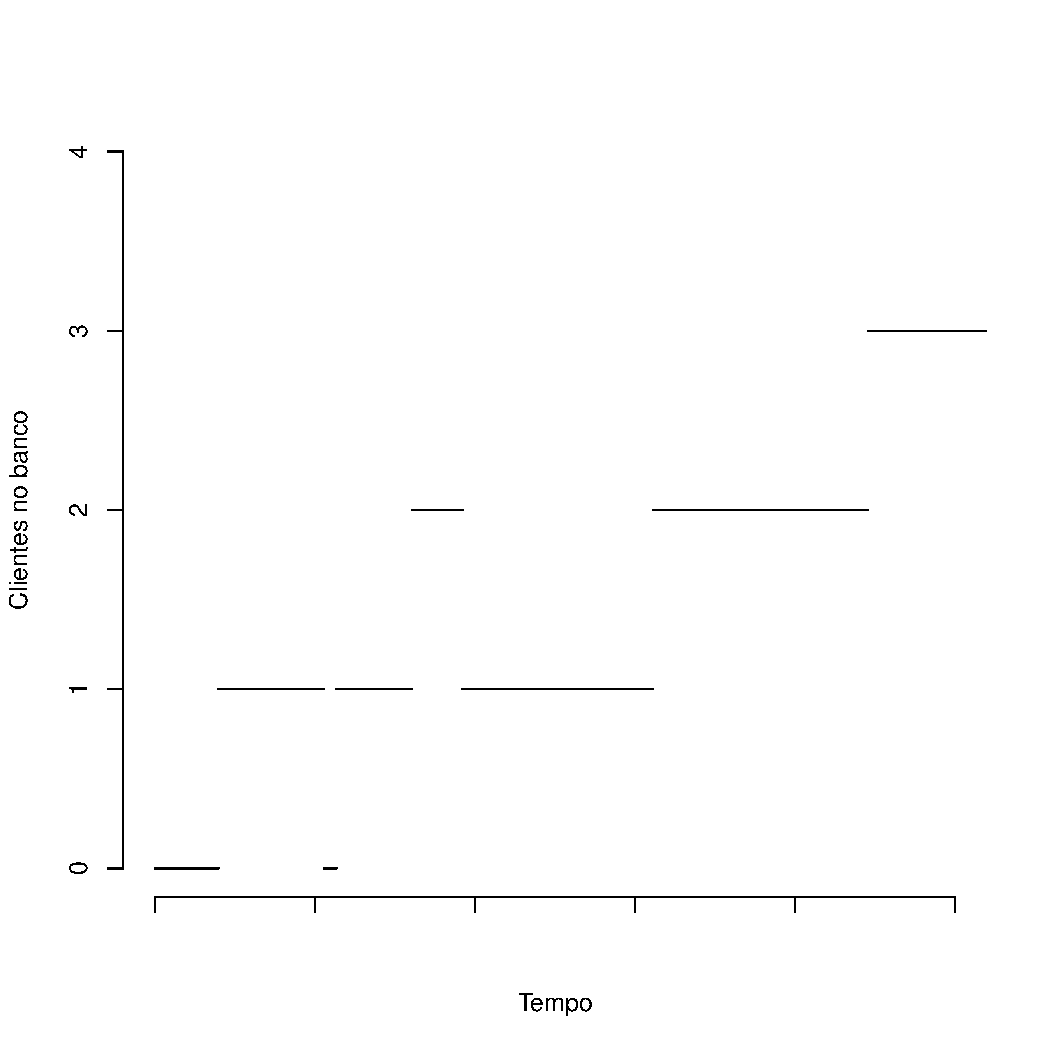
\includegraphics[width=0.8\textwidth,trim=0cm 0cm 0cm
    1.5cm]{fila.pdf}
  \end{center}
\end{frame}

\begin{frame}
  \begin{itemize}
  \item Funções aleatórias como essa são chamadas de processos
    estocásticos;
  \item Esse processo é em tempo contínuo;
  \item O conjunto dos valores que o processo pode assumir é chamado
    de espaço de estados, no caso da fila apresentada ele é $\{0, 1,
    2, \ldots\}$;
  \item Filas normalmente são processos não explosivos, o que não é o
    caso do Processo K.
  \end{itemize}
\end{frame}

\section{Definições e construção}

\subsection{Espaço de estados e parâmetros}

\begin{frame}

  Denota-se por $\Nz$ o conjunto dos números naturais positivos, isso
  é:
  \begin{displaymath}
    \Nz = \left\{ 1, 2, 3, \ldots \right\}.
  \end{displaymath}

  O Processo K é um processo estocástico em tempo contínuo construído
  sobre o espaço:
  \begin{displaymath}
    \Nzb = \Nz \cup \{ \infty \},
  \end{displaymath}

\end{frame}


\begin{frame}

  Associa-se duas constantes positivas à cada estado $x \in \Nz$ do
  processo:

  \begin{itemize}
  \item $\lambda_x$: controla a taxa em que tendemos a entrar em no
    estado $x$;
    
  \item $\gamma_x$: tempo médio em que permanecemos no estado $x$ em
    cada visita.
  \end{itemize}

  Considere ainda uma constante $c$ não negativa, que irá controlar 
  o tempo em que o processo passa no infinito.

\end{frame}

\begin{frame}

  Impõe-se duas restrições sobre esses parâmetros:
  \begin{block}{}
    \begin{enumerate}
    \item $ \displaystyle \sum_{x\in \Nz} \lambda_x \gamma_x <
      \infty $
      \bigskip
    \item $ \displaystyle \sum_{x\in \Nz} \lambda_x = \infty $
    \end{enumerate}
  \end{block}
\end{frame}

\subsection{Construção}

\begin{frame}

  O Processo K é construído num Espaço de Probabilidades que admita as
  seguintes famílias de variáveis aleatórias independentes:

  \begin{itemize}
  \item $\{ N_x: x \in \Nz\}$ : Processos de Poisson independentes,
    com taxas $\{ \lambda_x : x \in \Nz \}$;
  \item $\{T_0\} \cup \{ T_i^x: i, x \in \Nz  \}$ : variáveis aleatórias
    \emph{i.i.d.} com distribuição exponencial de média $1$.
  \end{itemize}

  Denota-se por $\sigma^x_1 < \sigma^x_2 < \ldots$ as marcas do
  Processo de Poisson $N_x$.
  
\end{frame}

\begin{frame}

  A construção do Processo K se baseia na seguinte função aleatória,
  definida sobre $t \in [0, \infty)$:

  \begin{displaymath}
    \Gamma(t) := \Gamma^y(t) :=
    \gamma_y T_0 + \sum_{x \in \Nz} \sum_{i = 1}^{N_x (t)} \gamma_x T^x_i + c t
  \end{displaymath}
\end{frame}

\begin{frame}
  
  O Processo K com estado inicial $y \in \Nzb$ é definido como:

  \begin{displaymath}
    X(t) := X^y (t) :=
    \begin{cases}
      y & \textrm{ se }  t < \gamma_y T_0\\
      x & \textrm{ se } \Gamma^y(\sigma_i^x-) \leq t <
      \Gamma^y(\sigma^x_i)
      \textrm{ para algum } i \\
      \infty & \textrm{ caso contrário.}
    \end{cases}
  \end{displaymath}
\end{frame}

\subsection{Exemplos}

\begin{frame}
  \begin{center}
    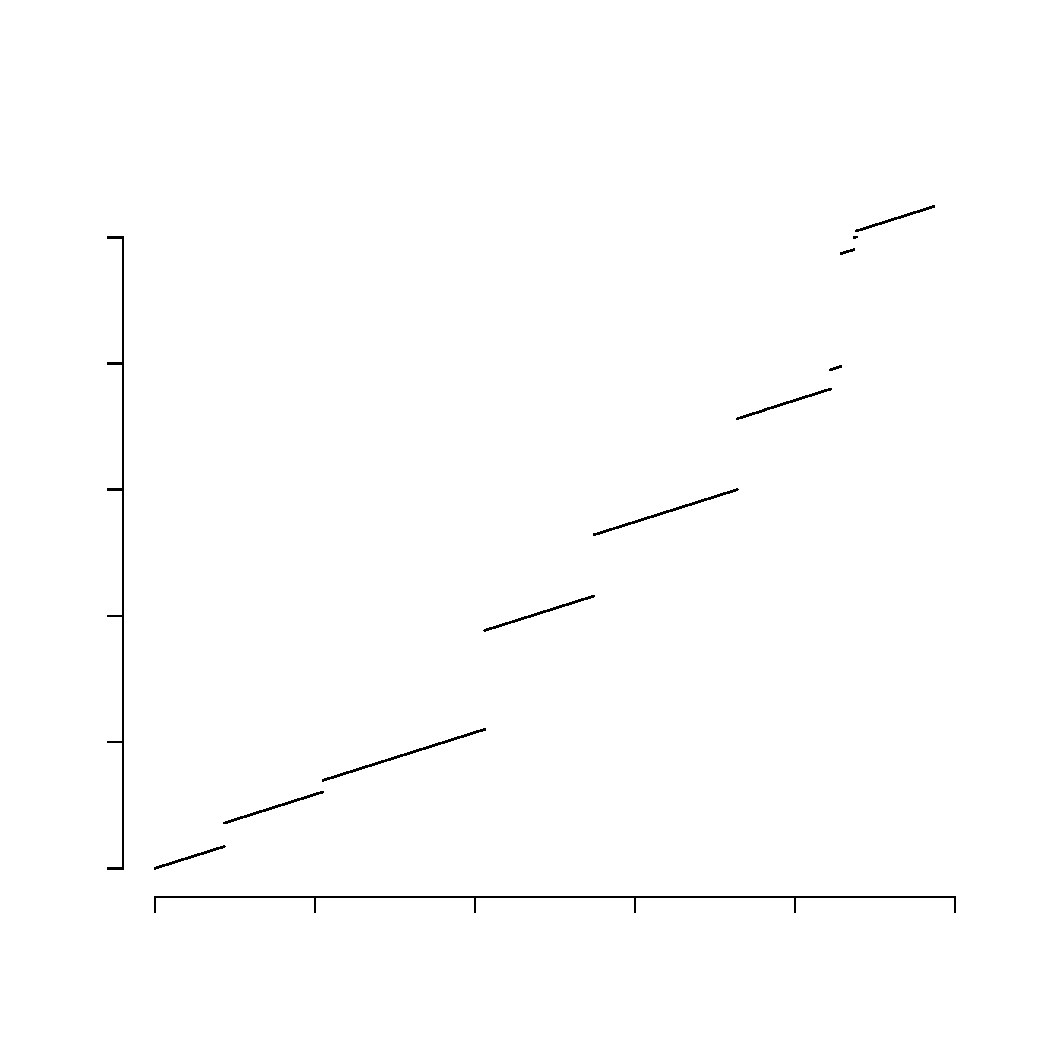
\includegraphics[width=\textwidth,trim=0cm 4.5cm 0cm 4.5cm]{gamma_c1}
  \end{center}
\end{frame}

\begin{frame}
  \begin{center}
    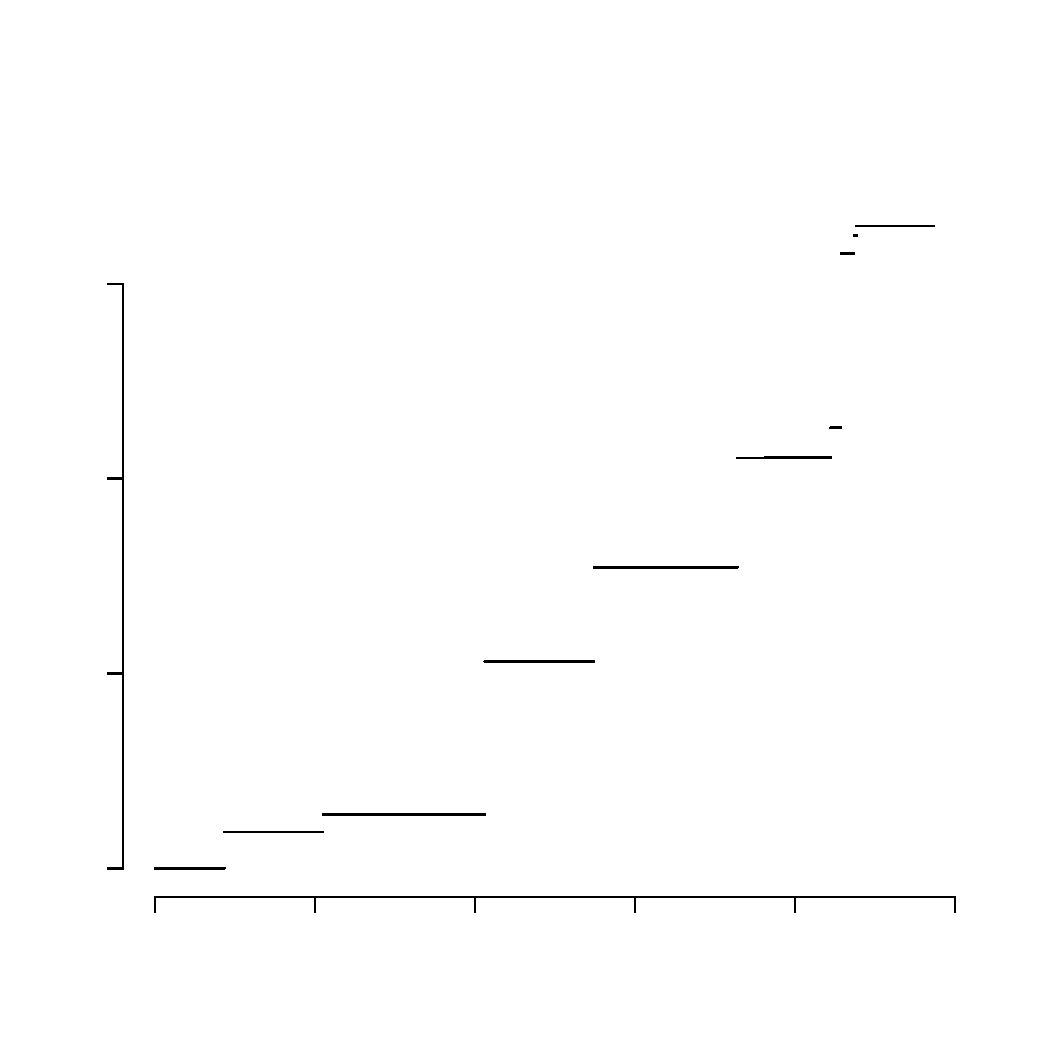
\includegraphics[width=\textwidth,trim=0cm 4.5cm 0cm 4.5cm]{gamma_c0}
  \end{center}
\end{frame}


\subsection{Topologia}

\begin{frame}
  
  Usaremos a seguinte métrica sobre $\Nzb$:
  \begin{displaymath}
    d(x, y) = \left\lvert \frac{1}{x} - \frac{1}{y} \right\rvert
  \end{displaymath}


  \begin{itemize}
  \item<2-> Todo ponto $x \in \Nz$ é um ponto isolado;
  \item<3-> Uma sequência converge para $\infty$ se ela divergir para o
    infinito da maneira usual.
  \item<4-> Essa métrica é {\bf completa};
  \item<5-> Gera uma topologia {\bf compacta};
  \item<6-> Uma função $f: \Nzb \to \R$ é contínua se e somente se:
    \begin{displaymath}
      f(\infty) = \lim_{x \to \infty} f(x) .
    \end{displaymath}
  \end{itemize}

\end{frame}

\section{Resultados}

\subsection{Processo truncado}

\begin{frame}

  Para cada $n \in \Nzb$  e $y \in \{ 1, \ldots, n\} \cup \{ \infty
  \}$ defini-se o processo truncado em $n$ com condição inicial $y$ da
  seguinte forma:


\begin{displaymath}
  \Gamma^{y,(n)}_c (t) = \gamma_y T_0
  + \sum_{x =1}^{n} \sum_{i = 1}^{N_x(t)}
  \gamma_x T_i^x
  + c t.
\end{displaymath}

\begin{displaymath}
   X^{y,(n)}_c(t) = \begin{cases}
    y, & \textrm{ se }  t < \gamma_y T_0 \\
    x, & \textrm{ se } \Gamma^{y,(n)}_c(\sigma_i^x-) \leq t <
    \Gamma^{y,(n)}_c(\sigma^x_i)
    \text{ para algum } i \\
    \infty, & \textrm{ caso contrário.}
  \end{cases}
\end{displaymath}
\end{frame}


\begin{frame}
  \begin{teorema}
    O processo truncado em $n$ converge para o Processo K quase
    certamente na métrica de Skorohod quando $n \to \infty$.
  \end{teorema}

  A métrica de Skorohod é uma métrica sobre as trajetórias cádlág que
  admite pequenas distorções temporais.
\end{frame}


\subsection{Propriedade de Feller}

\begin{frame}

  \begin{definicao}
    Para cada $t \in [0, \infty)$, o semigrupo de transição é um
    operador sobre as funções de $\Nzb$ em $\R$ definido como:
    \begin{displaymath}
      \Psi_t f (y) = \E \left[ f(X^y(t)) \right]
    \end{displaymath}
  \end{definicao} \pause

  \begin{teorema}
    São equivalentes:
    \begin{itemize}
    \item $\displaystyle \lim_{x \to \infty} \gamma_x = 0$.
    \item $\Psi_t f$ é uma função contínua para todo $t > 0$ e $f:
      \Nzb \to \R$ contínua;
    \end{itemize}
  \end{teorema}
\end{frame}

\begin{frame}

  O Processo K pode não apresentar a propriedade de Feller, porém
  podemos trabalhar quase como se a tivéssemos.


  \begin{block}{Intuição}
    Se $f: \Nzb \to \R$ é uma função contínua e $(y_n)_n$ for uma
    sequência de estados que convirja para $y$ e tais estados ``possam
    ser visitados'' pelo Processo K em tempo finito, então:
    \begin{displaymath}  
      \Psi_t f (y_n) \xrightarrow{n \to \infty} \Psi_t f (y)
    \end{displaymath}
  \end{block}
\end{frame}

\subsection{Propriedade de Markov}

\begin{frame}
  \begin{teorema}
    O Processo K é fortemente markoviano.
  \end{teorema}
\end{frame}


\subsection{Taxas de transição}

\begin{frame}
  \begin{definicao}
    Para $x, y \in \Nzb$ e $t > 0$, denota-se
    \begin{displaymath}
      p_{x y} (t) := P \left( X^x(t) = y \right).
    \end{displaymath}
    $P (t)$ denotará a matriz cujas entradas são $p_{x y} (t)$.
  \end{definicao} \pause
  \begin{definicao}
    A matriz de taxas de transição é definida como:
    \begin{displaymath}
      Q := \lim_{t \searrow 0} \frac{P(t) - I}{t},
    \end{displaymath}
    onde $I$ é a matriz identidade.
  \end{definicao}
\end{frame}

\begin{frame}
  \begin{teorema}
    No caso $c > 0$, a matriz de taxas de transição vale:
    \begin{displaymath}
      Q = \left(
        \begin{array}{ccccc}
          -1/\gamma_1 & 0 & 0 & \cdots & 1/\gamma_1\\
          0 & -1/\gamma_2 & 0 & \cdots & 1/\gamma_2\\
          0 & 0 & -1/\gamma_3 & \cdots & 1/\gamma_3\\
          \vdots & \vdots & \vdots & \ddots & \vdots \\
          \lambda_1/c & \lambda_2/c &
          \lambda_3/c & \cdots & -\infty\\
        \end{array}
      \right).
    \end{displaymath}
  \end{teorema}
\end{frame}

\begin{frame}
  \begin{teorema}
    No caso $c = 0$, a matriz de taxas de transição vale:
    \begin{displaymath}
      Q = \left(
        \begin{array}{ccccc}
          -1/\gamma_1 & 0 & 0 & \cdots & 0\\
          0 & -1/\gamma_2 & 0 & \cdots & 0\\
          0 & 0 & -1/\gamma_3 & \cdots & 0\\
          \vdots & \vdots & \vdots & \ddots & \vdots \\
          \infty & \infty & \infty & \cdots & -\infty\\
        \end{array}
      \right).
    \end{displaymath}
  \end{teorema}
\end{frame}

\subsection{Distribuição invariante}

\begin{frame}
  \begin{teorema}
    A única medida de probabilidade invariante do Processo K é dada
    por:
    \begin{displaymath}
      \pi(x) := \begin{cases}
        \frac{\lambda_x \gamma_x}{c + \sum_{y \in \Nz} \lambda_y \gamma_y}
        & \textrm{ se } x \in \Nz \\
        \frac{c}{c + \sum_{y \in \Nz} \lambda_y \gamma_y}
        & \textrm{ se } x = \infty \\
      \end{cases}
    \end{displaymath}
  \end{teorema}
\end{frame}

\subsection{Tempo no infinito}

\begin{frame}

  Considere o conjunto dos instantes de tempo que o Processo K, passa
  no infinito, isso é:
  \begin{displaymath}
    \RR = \left\{ t \geq 0: X^\infty(t) = \infty \right\}
  \end{displaymath}
  \pause
  \begin{teorema}
    A medida de Lebesgue de $\RR$ vale zero \qc quando $c = 0$.
  \end{teorema}
  \begin{teorema}
    A medida de Lebesgue de $\RR$ é positiva \qc quando $c > 0$.
  \end{teorema}
\end{frame}

\begin{frame}
  \begin{teorema}
    Quando $c = 0$, denotando por $\dim_H (A)$ a dimensão de Hausdorff
    de um conjunto $A$, para todo $t > 0$ vale que quase certamente:
    \begin{displaymath}
      \dim_H(\RR \cap [0, t]) = 
      \liminf_{u \to \infty} 
      \frac{1}{\log u} \log \left(
        \sum_{x \in \Nz} \frac{u \lambda_x \gamma_x}{1 + u\gamma_x}
      \right).
    \end{displaymath}
  \end{teorema}
\end{frame}

\begin{frame}

  \begin{teorema}
    Supondo que $\sup_{x\in\Nz}\lambda_x < \infty$ e que existam um
    $\delta>0$ e um $n_0 \in \Nz$ tal que $\gamma_x \leq
    x^{-(1+\delta)}$ para todo $x > n_0$, vai valer que:
    \begin{displaymath}
      \dim_H(\RR \cap [0, t]) \leq \frac{1}{1+\delta} .
    \end{displaymath}
  \end{teorema}

  \begin{teorema}
    Supondo que $\inf_{x\in\Nz}\lambda_x > 0$ e que existam um
    $\delta>0$ e um $n_0 \in \Nz$ tal que $\gamma_x \geq
    x^{-(1+\delta)}$ para todo $x > n_0$, vai valer que:
    \begin{displaymath}
      \dim_H(\RR \cap [0, t]) \geq \frac{1}{1+\delta} .
    \end{displaymath}
  \end{teorema}
\end{frame}

\subsection{Gerador infinitesimal}

\begin{frame}

  Iremos nos limitar ao caso homogêneo, isso é, $\lambda_x = 1$ para
  todo $x \in \Nz$.

  \begin{definicao}
    O gerador infinitesimal $\AAA$ calculado sobre uma função $f: \Nzb
    \to \R$ é definido pelo limite:
    \begin{displaymath}
      \AAA f (x) = \lim_{t \searrow 0} \frac{\Psi_t f (x) - f(x)}{t}.
    \end{displaymath}
  \end{definicao}
  
  Note que esse limite pode não existir.

\end{frame}  


\begin{frame}
  \cite{kendall:56} calcularam o gerador no caso $c = 1$.

  \begin{teorema}
  Para uma função $f: \Nzb \to \R$ tal que
  \begin{displaymath}
    \lim_{x \to \infty}
    \frac{f(x) - f(\infty)}{\gamma_x} = \sum_{x \in \Nz}
    [f(\infty) - f(x)]
  \end{displaymath}
  vale que:
  \begin{displaymath}
    \AAA f (x) = \begin{cases}
      \displaystyle
      \frac{f(\infty) - f(x)}{\gamma_x} & \text{se } x \in \Nz\\
      \displaystyle
      \sum_{y\in \Nz} [f(y) - f(\infty)] & \text{se } x = \infty.
    \end{cases}
  \end{displaymath}
\end{teorema}
\end{frame}

\begin{frame}

  Quando $c = 0$, o domínio onde iremos definir o gerador será 
  o conjunto $\DDD$ das funções $f: \Nz \to \R$ tais que:

  \begin{itemize}
  \item $\displaystyle \lim_{x \to \infty} \frac{f(x) -
      f(\infty)}{\gamma_x}$ existe
  \item $\displaystyle \sum_{x\in \Nz} |f(x)-f(\infty)| < \infty$
  \item $\displaystyle \sum_{x\in \Nz} \left( f(x)-f(\infty)\right) = 0$
  \end{itemize}  
\end{frame}

\begin{frame}

  \begin{teorema}
    Quando $c = 0$, para $f \in \DDD$, vale que:
    \begin{displaymath}
      \AAA f (x) = \begin{cases}
        \displaystyle
        \frac{f(\infty) - f(x)}{\gamma_x} & \text{ se } x \in \Nz \vspace{2mm}\\
        \displaystyle
        \lim_{y \to \infty} \frac{f(y) - f(x)}{\gamma_x} & \text{ se } x=\infty\\
      \end{cases}
    \end{displaymath}
  \end{teorema}
  \pause
  \begin{teorema}
    A função $\AAA$, definida acima é um gerador infinitesimal que
    caracteriza o semigrupo $\Psi_t$.
  \end{teorema}
\end{frame}



\begin{frame}[plain]
  \frametitle{Referências}
  \bibliographystyle{plainnat} 
  \bibliography{../bibliografia} 
\end{frame}

\end{document}

%%% Local Variables: 
%%% mode: latex
%%% TeX-master: t
%%% End: 
